姿态控制器使用级联回路方法工作, 如图\ref{atti}所示。外环计算姿态设定值和估计姿态之间的误差,该误差乘以增益(P控制器)可生成速率设定点。然后,内部循环计算速率误差,并使用PI(比例+积分)控制器生成所需的角加速度。
然后,使用此期望的角加速度和通过控制分配(也称为混合)对系统的先验知识,计算控制执行器(飞机,电梯,舵等)的角位置。此外,由于控制面在高速时更有效,而在低速时则较差,因此使用空速测量(如果使用此类传感器)来缩放针对巡航速度进行调整的控制器。
如果未使用空速传感器,则会禁用FW姿态控制器的增益调度(它是开环的);使用空速反馈在TECS中无法/无法进行校正。
\par前馈增益用于补偿空气动力学阻尼。基本上,飞机上机轴力矩的两个主要组成部分是由控制面(飞机,电梯,方向舵,产生运动)和气动阻尼(与机率成比例,抵消运动)产生的。为了保持恒定的速率,可以使用速率环路中的前馈来补偿此阻尼。
侧倾和俯仰控制器具有相同的结构,并且假定纵向和横向动力学已解耦到足以独立工作。但是,偏航控制器使用转角协调约束来生成其偏航率设定值,以最小化飞机滑行时产生的横向加速度。偏航率控制器还有助于抵消不利的偏航影响,并通过提供额外的定向阻尼来阻尼荷兰语侧倾模式。
        \begin{figure}[t]
            \centering
            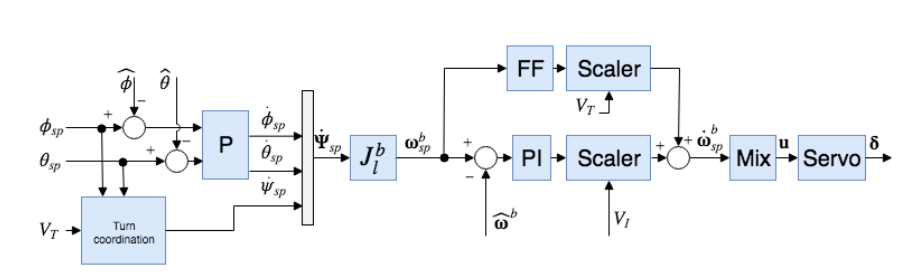
\includegraphics[width=0.7\textwidth]{pictures/attitude.png}
            \caption{attitude control loop}
            \label{atti}
        \end{figure}